\documentclass[../main/report.tex]{subfiles}
\begin{document}
\begin{figure}[H]
	\centering
	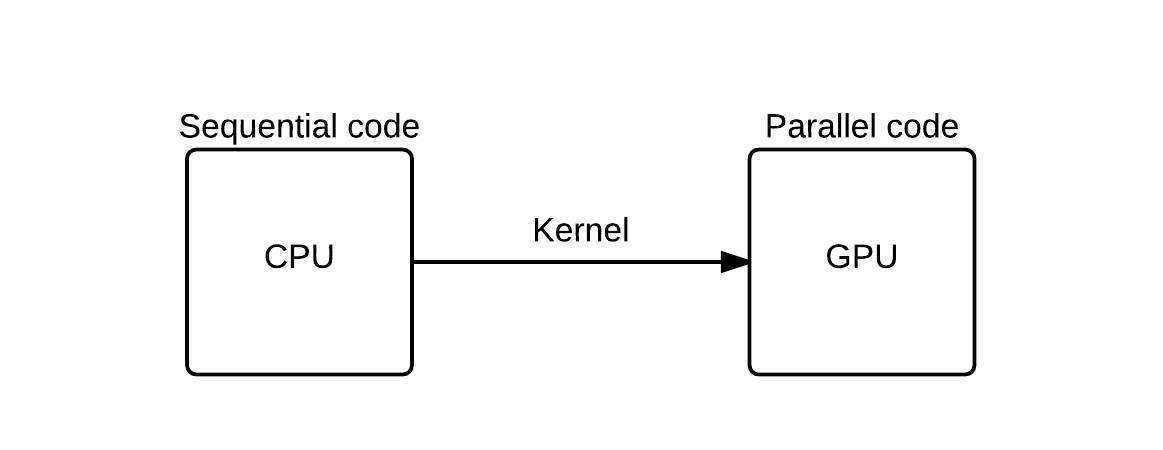
\includegraphics[width=\textwidth]{../system_overview/diagrams/programming_model_cpu_gpu.png}
	\caption{Relationship between CPU and GPU code.}
	\label{fig:programming_model_cpu_gpu}
\end{figure}

The programming model for Demolicious is heavily inspired by CUDA.

So let's see how we can implement the same program filling a framebuffer with green, as we did in the CUDA introduction in section \ref{sec:cuda_prog_model}.

Below, in listing \ref{lst:green-kernel}, the fillscreen kernel has been converted for the Demolicious programming paradigm.
The first thing you'll notice is that it is not written in C, but assembly.
The complete introduction to the Demolicious instruction set and assembly programming can be found in appendix \ref{chap:isa}.

\begin{assembly}[caption=A simple kernel that fills the screen with the color green, label=lst:green-kernel]
ldi $data, 0b0000011111100000
mv $address_lo, $id_lo
mv $address_hi, $id_hi
sw
thread_finished
\end{assembly}

Let's walk through the kernel one line at a time.

The first line uses the \verb/ldi/ instruction, which stands for load immediate.
It loads the value 0b0000011111100000,
which corresponds to the color green in the Demolicious color space,
into the special register \textbf{\$data}.

The second and third line move the kernel's thread ID into the address registers.

Finally, the store instruction is executed, storing the value in the \textbf{\$data} register
to the address given by the two address registers.
This means all pixels starting with address zero and up until the number of executed threads
will get colored green.

The thread stops running after executing the \verb/thread_finished/ instruction.

\subsection{Executing Kernels}

Now, how do we execute this kernel on the GPU?
The program running on the CPU, referred to as the \emph{host program},
has to upload the assembled kernel to the GPU, and then tell the GPU to run it.
Kernels can be assembled using the provided assembler\ref{sec:assembler}.

\begin{c-code}[caption=Loading and executing a kernel, label=lst:load-kernel]
instruction_t fill_screen_kernel[] = {
    0x08050000, // ldc $data, 0
    0x00402004, // mv $address_lo, $id_lo
    0x00201804, // mv $address_hi, $id_hi
    0x10000000, // sw
    0x40000000 // thread_finished
};

kernel_t fill_screen = load_kernel(fill_screen_kernel);

run_kernel(fill_screen, 4096);
\end{c-code}

In listing \ref{lst:load-kernel}, we first see the assembled kernel stored in the
\verb/fill_screen_kernel/ array.
It is then uploaded to the GPU using the \verb/load_kernel/ function.
A reference to the uploaded kernel is returned, which will be used when starting the kernel.
In addition, the \verb/run_kernel/ function is also provided with the number of threads to spawn.
Here, we spawn 4096 threads, enough to color 64*64 pixels green.

A difference from the CUDA programming model is that on Demolicious, kernels can access the actual framebuffers directly.
So while you had to read back the framebuffer from the GPU memory in CUDA to visualize it,
this kernel writes directly to one of the framebuffers \footnote{see double buffering? @ref or elaborate@} that is being shown on screen through HDMI.

While being able to make the screen green by running a specialized kernel is nice,
it would require many similar kernels to color the screen in different colors.
To improve on this, kernels can take parameters as input,
which lets them be reused with varying output.
The CPU can set these parameters to different values each time a kernel is run.
For instance, the CPU can set the desired color as a parameter,
and the kernel will store that value to memory instead of a predefined immediate.
Listing \ref{lst:param-color-kernel} shows an example kernel where the color is stored as a parameter.

\begin{assembly}[caption=A kernel loading the color value from a parameter, label=lst:param-color-kernel]
ldc $data, 0
mv $address_lo, $id_lo
mv $address_hi, $id_hi
sw
thread_finished
\end{assembly}

The only changed line in this kernel is the first one,
where instead of using an immediate value, we load a value using the \verb/ldc/ (load constant) instruction.
The value is a constant from the kernel's viewpoint, as it cannot be changed from the GPU.
Instead, the value is set from the CPU using the \verb/load_constant/ function,
as seen in listing \ref{lst:kernel-constant}.

\begin{c-code}[caption=Now drawing a blue screen using parameters, label=lst:kernel-constant]
load_constant(0, 0x001F);
run_kernel(fill_screen, 4096);
\end{c-code}

\subsection{More Advanced Kernels}
The instruction set available to kernels is fairly limited.
Most notably, the control flow in kernels is linear, meaning they cannot do any branches or jumps. See section \label{sec:demolicious-demo-machine} for more detail.

Although the kernels don't support diverging control flow,
conditional execution is accomplished through predicated instructions.

Each of the instructions in the instruction set (except for loads and stores) can be executed conditionally by prefixing them with '\textbf{?}'.
Whether a conditional instruction is executed is controlled by a dedicated mask register.
The programmer may use arithmetic and logic operations to manipulate this register (such as the \verb/srl/ instruction on line 3 in listing \ref{lst:masked-execution}).
The result of a predicated instruction will be discarded if the mask register is \textbf{1}.

\begin{assembly}[caption=Conditional execution using predicated instructions, label=lst:masked-execution]
ldc $10, 0 ; Load color one
ldc $11, 1 ; Load color two
srl $mask, $id_lo, 6 ; Shift to the right converts ID to y pos
mv $data, $10 
? mv $data, $11 ; Will only be executed every other row
mv $address_lo, $id_lo
mv $address_hi, $id_hi
sw
thread_finished
\end{assembly}

The kernel starts by loading two color parameters.
It then stores a shifted thread ID into the mask register.
Shifting a thread ID to the right is a trick to convert the ID to a y value,
which works when the screen width is a power of two.
The mask register is only 1 bit, and will just store the least significant bit written to it.
This means that masking will be enabled for odd rows and disabled for even rows.
Line 4 first writes a color value to the \textbf{\$data} register.
When masking is disabled this value will be overwritten on line 5.
The kernel finishes by writing the data value to memory.

This section contains some simplifications, namely some \verb/nop/ instructions that are required under some specific circumstances have been omitted.
The actual kernel code that is sent to the GPU for the kernel that fills the screen with green,
can be seen in listing \ref{lst:real-green-kernel}.
The kernel from listing \ref{lst:masked-execution} however, is executed as is. The reason for these \verb/nop/ instructions will be explained in later chapters.

\todo{Finish the nop examples}
\begin{assembly}[caption=The green-screen kernel as it is actually , label=lst:real-green-kernel]
ldi $data, 0b0000011111100000
mv $address_lo, $id_lo
mv $address_hi, $id_hi
sw
nop
nop
nop
thread_finished
\end{assembly}

As illustrated by these examples, while the kernels on Demolicious are more limited than CUDA kernels, the programming models are very similar.
With these examples in mind, it's time to take a look behind the scenes and see how the CPU and GPU actually run this code.

\end{document}
